\chapter{Resultados}
\label{cap:pruebas}

Este capítulo presenta los resultados obtenidos con el sistema implementado
en el capítulo~\ref{cap:implementacion}: la comparativa de ByteTrack y
OC-SORT sobre entrenamiento y test, el efecto del estudio de
hiperparámetros, y los resultados del pipeline de metadatos sobre las secuencias de
demostración. El capítulo dedica una atención especial a la distinción
entre HOTA y HOTA(0) introducida en la
sección~\ref{subsec:impl-hota-vs-hota0}, ya que cambia de forma sustancial la conclusión comparativa entre
ambos algoritmos. El capítulo se cierra con una discusión
consolidada de las limitaciones de todos los resultados presentados.

\section{Descripción de experimentos}
\label{sec:pruebas-config}

Todos los resultados de este capítulo se han obtenido con la configuración
descrita en el capítulo~\ref{cap:implementacion}: \texttt{TrackEval}
configurado con \texttt{BENCHMARK='SoccerNet'} y
\texttt{THRESHOLD=0.5} (sección~\ref{sec:implementacion-evaluacion}),
sobre las 57 secuencias del conjunto de entrenamiento y las 44 del
conjunto de test de SoccerNet-Tracking. Por cada
combinación de algoritmo y split se reportan tres métricas
(HOTA, MOTA e IDF1 (sección~\ref{sec:fundamentos-metricas})),
y
adicionalmente HOTA(0) allí donde la distinción con HOTA integrada es
relevante para la lectura correcta del resultado.

\section{Estrategia de validación}
\label{sec:pruebas-estrategia}

La comparación entre algoritmos se apoya en dos evaluaciones con propósitos
distintos: una
primera evaluación sobre el conjunto de \textbf{entrenamiento}, obtenida
durante el desarrollo inicial y usada para validar que el pipeline de
tracking y evaluación funcionaba correctamente, y una
segunda evaluación sobre el conjunto de \textbf{test}, realizada para
sustentar las conclusiones comparativas de este capítulo.
Ninguna decisión de diseño ni de hiperparámetros se ha tomado consultando
los resultados de test antes de esta evaluación final, de modo que el
conjunto de test se comporta como datos no vistos.

\section{Comparativa de algoritmos: ByteTrack frente a OC-SORT}
\label{sec:pruebas-comparativa}

La Tabla~\ref{tab:pruebas-comparativa} recoge los resultados de ambos
algoritmos, en su configuración por defecto (sin el ajuste de
hiperparámetros de la sección~\ref{sec:pruebas-hiperparametros}), sobre
entrenamiento y test.

\begin{table}[htp]
\centering
\caption{Resultados de ByteTrack y OC-SORT sobre entrenamiento y test con la configuración por defecto.}
\label{tab:pruebas-comparativa}
\renewcommand{\arraystretch}{1.25}
\begin{tabular}{|p{1.7cm}|p{2.1cm}|p{1.3cm}|p{1.8cm}|p{1.3cm}|p{1.3cm}|p{1.3cm}|p{1.3cm}|}
\hline
\rowcolor{gray!25}
\textbf{Split} & \textbf{Algoritmo} & \textbf{HOTA} & \textbf{HOTA(0)} & \textbf{DetA} & \textbf{AssA} & \textbf{MOTA} & \textbf{IDSW} \\
\hline
\multirow{2}{*}{Train} & ByteTrack & 73.27 & 82.97 & 81.59 & 65.86 & 92.15 & 3\,866 \\
\cline{2-8}
 & OC-SORT & \textbf{80.23} & 80.34 & \textbf{92.11} & \textbf{69.88} & 92.01 & \textbf{2\,205} \\
\hline
\multirow{2}{*}{Test} & ByteTrack & 70.73 & 80.20 & 80.54 & 62.18 & \textbf{90.78} & 5\,561 \\
\cline{2-8}
 & OC-SORT & \textbf{75.43} & 75.51 & \textbf{87.23} & \textbf{65.22} & 87.01 & \textbf{2\,046} \\
\hline
\end{tabular}
\end{table}

La lectura inmediata de la columna HOTA, la métrica integrada y más
completa de las tres empleadas en este proyecto
(sección~\ref{subsec:fundamentos-hota}) es clara: \textbf{OC-SORT supera
a ByteTrack tanto en entrenamiento como en test}, tanto en detección
(DetA) como en asociación (AssA), y con considerablemente menos cambios de
identidad (IDSW). Solo en MOTA la métrica más sesgada hacia la
detección y menos exigente con la asociación ByteTrack iguala o supera
ligeramente a OC-SORT.

\subsection{Por qué HOTA y HOTA(0) son distintas}
\label{subsec:pruebas-hota-explicacion}

La columna HOTA(0) de la Tabla~\ref{tab:pruebas-comparativa} tiene como valor de
HOTA en el único umbral IoU de 0,5, en lugar de integrado sobre el rango
completo (sección~\ref{subsec:impl-hota-vs-hota0}) cuenta una historia
distinta y, en test, directamente contraria: bajo HOTA(0), ByteTrack
(80,20) supera claramente a OC-SORT (75,51). Es precisamente esta lectura
la que se usó, sin advertirlo explícitamente en su
momento, en las anotaciones de seguimiento de este proyecto durante el
desarrollo, y la que llevó a concluir entonces que \emph{``en test los
resultados se invierten a favor de ByteTrack''}. La
Figura~\ref{fig:pruebas-hota-vs-hota0} contrasta ambas lecturas.

\begin{figure}[htp]
\centering
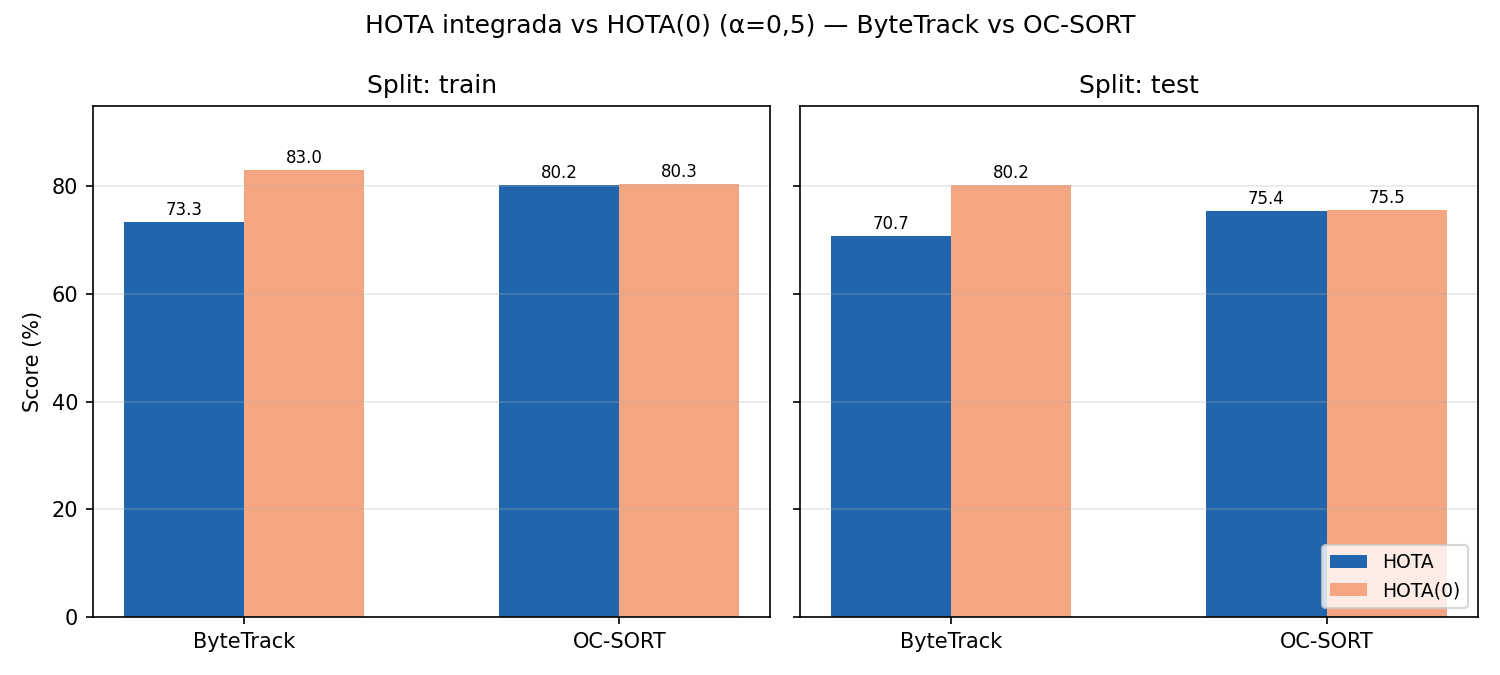
\includegraphics[width=0.92\textwidth]{figures/pruebas_hota_vs_hota0.png}
\caption{HOTA integrada frente a HOTA(0) para ambos algoritmos. Bajo HOTA
integrada, OC-SORT gana en ambos splits; bajo HOTA(0), la lectura se
invierte a favor de ByteTrack.}
\label{fig:pruebas-hota-vs-hota0}
\end{figure}

Esta discrepancia es visible en las columnas de
precisión de localización (\texttt{LocA}) del fichero
\texttt{pedestrian\_summary.txt} de \texttt{TrackEval}. OC-SORT alcanza una
\texttt{LocA} y una \texttt{DetPr} prácticamente perfectas (superiores al
99,9\,\% en ambos splits), lo que indica que \textbf{OC-SORT reutiliza
directamente las cajas del \texttt{det.txt} original sin modificarlas},
coherente con su diseño centrado en la observación. ByteTrack, en cambio, obtiene
una \texttt{LocA} sensiblemente más baja (89,8\,\% en train, 89,7\,\% en
test), lo que indica que sus cajas de salida se desvían algo más de las
detecciones originales (posiblemente por la interpolación de posición
que realiza el filtro de Kalman durante su segunda ronda de asociación con
detecciones de baja confianza (sección~\ref{subsec:fundamentos-bytetrack})).

Esa imprecisión de localización de ByteTrack apenas penaliza a HOTA(0),
calculada en un único umbral de IoU (0,5), pero se
paga cara en la HOTA integrada, que promedia también sobre umbrales mucho
más exigentes (hasta 0,95). A esos umbrales estrictos, una caja
ligeramente desplazada dejará de solapar lo suficiente con el
\emph{ground truth} para contar como acierto, mientras que las cajas casi
perfectas de OC-SORT siguen acertando. En definitiva, \textbf{ByteTrack
detecta más objetos y con más consistencia de identidad relativa
(mayor \texttt{DetRe}), pero los localiza con menos precisión. OC-SORT
detecta algo menos pero con una fidelidad casi perfecta a la detección
original}, y es esta diferencia de precisión geométrica, 
la que explica el por qué la métrica más exigente (HOTA integrada)
favorece a OC-SORT mientras que la métrica de umbral único (HOTA(0))
favorece a ByteTrack.

La conclusión que se extrae de esto y que corrige la lectura
inicial de las anotaciones de desarrollo de este proyecto, es que
\textbf{OC-SORT es el algoritmo con mejor rendimiento global en este
dataset}, tanto en entrenamiento como en test, cuando se evalúa con la
métrica íntegra y más robusta del campo. Dicho esto, ByteTrack con su menor precisión de localización es
perfectamente compatible con aplicaciones menos exigentes en exactitud
geométrica de la caja, y su comportamiento bajo ajuste de hiperparámetros
resulta, de hecho, más estable que el de OC-SORT.

\section{Resultados del estudio de hiperparámetros}
\label{sec:pruebas-hiperparametros}

El estudio de hiperparámetros se reporta en términos de HOTA(0) y no de
HOTA integrada. La Figura~\ref{fig:pruebas-hiperparametros} muestra el
efecto de los dos hiperparámetros con mayor impacto observado, uno por
algoritmo, y la Tabla~\ref{tab:pruebas-hiperparametros-sensibilidad}
recoge el análisis de sensibilidad completo sobre las configuraciones
base descritas en la sección~\ref{sec:implementacion-hiperparametros}.

\begin{figure}[htp]
\centering
\begin{minipage}{0.48\textwidth}
\centering
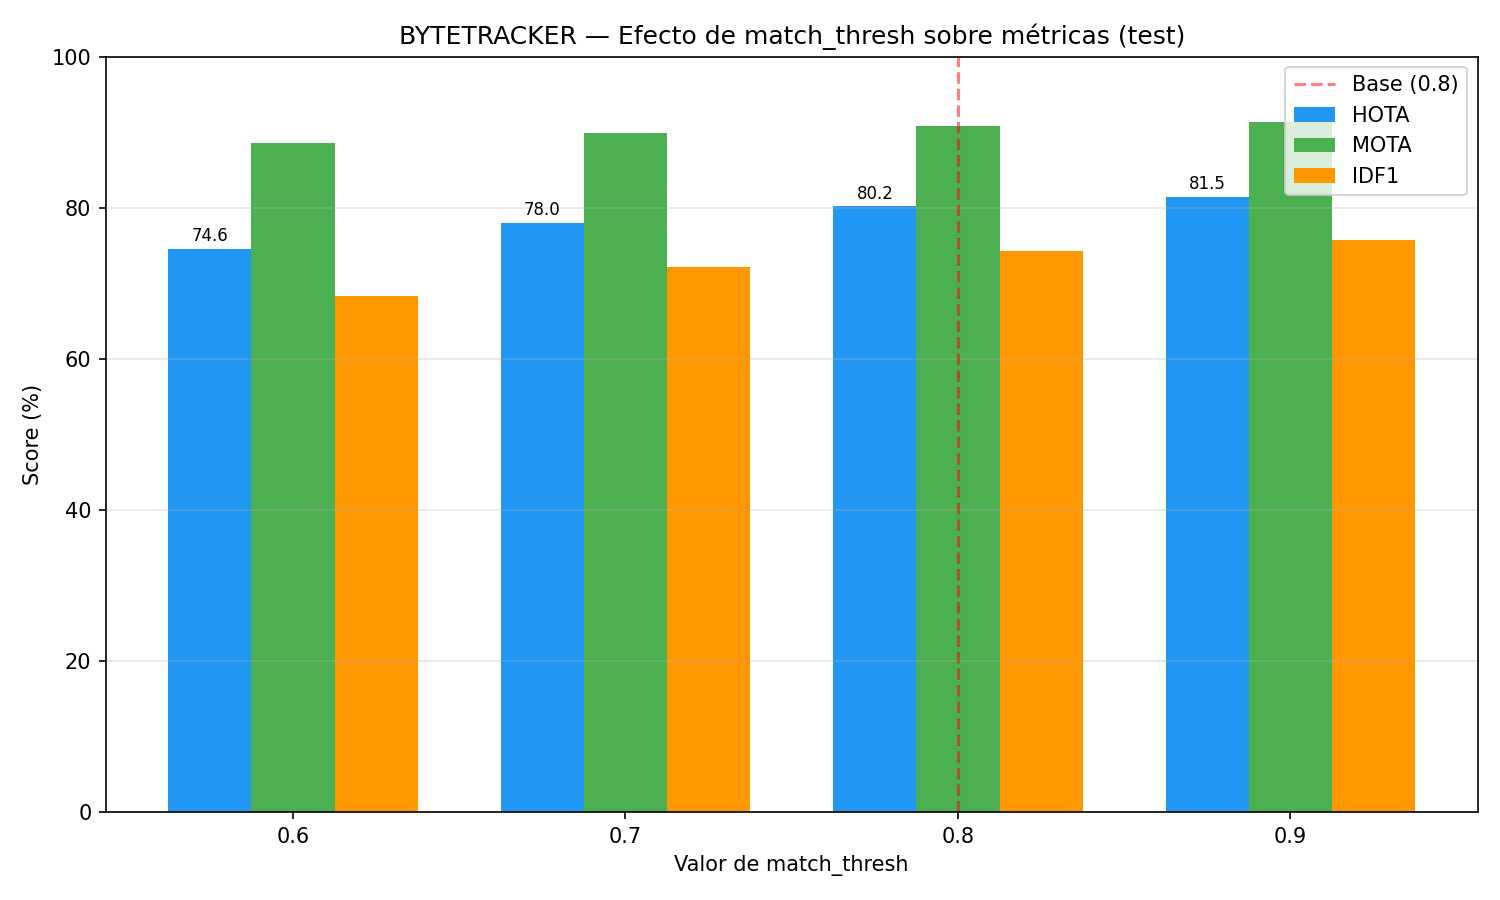
\includegraphics[width=\textwidth]{figures/pruebas_hiperparam_bytetracker.png}
\end{minipage}
\hfill
\begin{minipage}{0.48\textwidth}
\centering
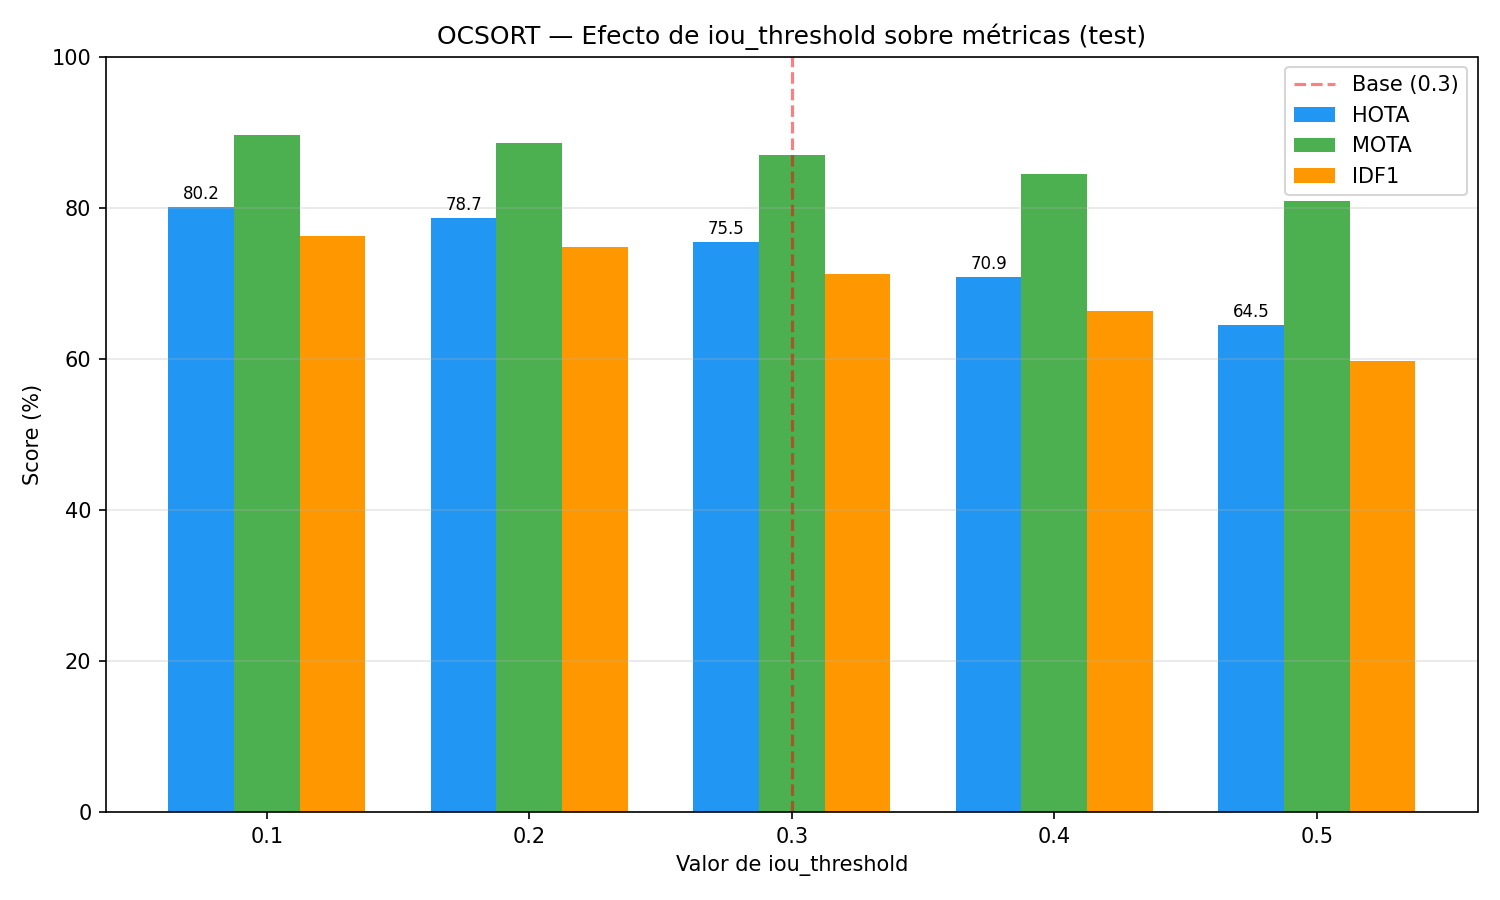
\includegraphics[width=\textwidth]{figures/pruebas_hiperparam_ocsort.png}
\end{minipage}
\caption{Efecto de \texttt{match\_thresh} sobre ByteTrack (izquierda) y de
\texttt{iou\_threshold} sobre OC-SORT (derecha), los dos hiperparámetros de
mayor impacto individual encontrados en el estudio
(sección~\ref{sec:implementacion-hiperparametros}).}
\label{fig:pruebas-hiperparametros}
\end{figure}

\FloatBarrier

\begin{table}[htp]
\centering
\caption{Análisis de sensibilidad: efecto de cada hiperparámetro sobre HOTA(0) (\%) en el conjunto de test.}
\label{tab:pruebas-hiperparametros-sensibilidad}
\renewcommand{\arraystretch}{1.2}
\small
\begin{tabular}{|p{3.1cm}|p{1.5cm}|p{1.5cm}|p{1.5cm}|p{1.5cm}|p{1.5cm}|}
\hline
\rowcolor{gray!25}
\textbf{Hiperparámetro} & \multicolumn{5}{c|}{\textbf{Valor del hiperparámetro}} \\
\hline
\texttt{match\_thresh} (BT) & 0.6 & 0.7 & 0.8 (base) & 0.9 & -- \\
\hline
HOTA(0) & 74.62 & 78.03 & 80.20 & \textbf{81.48} & -- \\
\hline
\texttt{track\_buffer} (BT) & 10 & 20 & 25 (base) & 40 & -- \\
\hline
HOTA(0) & \textbf{80.36} & 80.26 & 80.20 & 80.12 & -- \\
\hline
\texttt{iou\_threshold} (OC) & 0.1 & 0.2 & 0.3 (base) & 0.4 & 0.5 \\
\hline
HOTA(0) & \textbf{80.17} & 78.71 & 75.51 & 70.90 & 64.49 \\
\hline
\texttt{max\_age} (OC) & 10 & 20 & 30 (base) & 50 & -- \\
\hline
HOTA(0) & \textbf{76.13} & 75.75 & 75.51 & 75.13 & -- \\
\hline
\texttt{min\_hits} (OC) & 1 & 2 & 3 (base) & 5 & -- \\
\hline
HOTA(0) & \textbf{76.26} & 75.90 & 75.51 & 74.78 & -- \\
\hline
\end{tabular}
\end{table}

\FloatBarrier

El resultado más relevante de este estudio es que \textbf{el ajuste
de hiperparámetros beneficia mucho más a OC-SORT que a ByteTrack}: OC-SORT
mejora su HOTA(0) en test de 75,51 a 80,92 (+5,41 puntos) con la
configuración óptima combinada, mientras que ByteTrack mejora de 80,20 a
81,43 (+1,23 puntos). Dicho de otro modo, ByteTrack ya operaba cerca de su
óptimo con los valores por defecto, mientras que OC-SORT
requería un ajuste explícito para desplegar todo su rendimiento. Esta
observación es coherente con la comparativa de la
sección~\ref{sec:pruebas-comparativa}: si se repitiera la comparación de
HOTA integrada usando las configuraciones óptimas de ambos algoritmos en
lugar de sus valores por defecto, es razonable esperar que la ventaja de
OC-SORT sobre ByteTrack se mantenga o incluso se ampliase, dado que es
OC-SORT quien más partido saca del ajuste.

Es interesante notar que la configuración combinada de ByteTrack
(81{,}43) resulta ligeramente \emph{inferior} al mejor valor individual de
\texttt{match\_thresh} por sí solo (81{,}48 con
\texttt{match\_thresh=0.9} y \texttt{track\_buffer} sin modificar): los
efectos de ambos hiperparámetros no son estrictamente aditivos, y combinar
el mejor valor de cada uno por separado no garantiza el mejor resultado
conjunto. En OC-SORT, en cambio, la combinación de los tres
hiperparámetros (80{,}92) mejora claramente sobre cualquiera de ellos por
separado (mejor individual: 80{,}17 con \texttt{iou\_threshold=0.1}), lo
que indica que en este caso sí se refuerzan entre sí.

Por ser la configuración de mayor HOTA(0) absoluto entre las dos
configuraciones óptimas (81,43 frente a 80,92), \textbf{ByteTrack con
\texttt{match\_thresh=0.9} y \texttt{track\_buffer=10}} es la que se ha
usado como base de todo el pipeline de metadatos de la siguiente sección,
una decisión tomada en su momento con la información de HOTA(0) disponible
entonces.

\section{Resultados del pipeline de metadatos}
\label{sec:pruebas-metadatos}

Esta sección presenta los resultados del pipeline de metadatos sobre las secuencias de
demostración SNMOT-116, SNMOT-117 y SNMOT-118, obtenidos sobre la
configuración óptima de ByteTrack.

\subsection{Clasificación de equipos}

La Tabla~\ref{tab:pruebas-equipos} resume el resultado de la clasificación
de equipos por K-means (sección~\ref{subsec:impl-equipos}) sobre las tres
secuencias de demostración.

\begin{table}[htp]
\centering
\caption{Resultado de la clasificación de equipos por secuencia.}
\label{tab:pruebas-equipos}
\renewcommand{\arraystretch}{1.25}
\begin{tabular}{|p{2.2cm}|p{2.2cm}|p{2.2cm}|p{2.2cm}|}
\hline
\rowcolor{gray!25}
\textbf{Secuencia} & \textbf{Jugadores clasificados} & \textbf{Equipo 0} & \textbf{Equipo 1} \\
\hline
SNMOT-116 & 61 & 29 & 32 \\
\hline
SNMOT-117 & 46 & 16 & 30 \\
\hline
SNMOT-118 & 44 & 24 & 20 \\
\hline
\end{tabular}
\end{table}

\FloatBarrier

La verificación visual (\texttt{team\_visualization.py}) confirma que la
separación por color de camiseta funciona correctamente para los
jugadores de ambos equipos en las tres secuencias, como muestra la
Figura~\ref{fig:pruebas-teams}. Como se documentó en la
sección~\ref{sec:fundamentos-kmeans}, ningún \texttt{track\_id} queda
etiquetado como ``árbitro'': con $k=2$, el árbitro presente en la secuencia
se asigna incorrectamente al equipo de color más cercano al de su
uniforme, una limitación conocida.

\begin{figure}[htp]
\centering
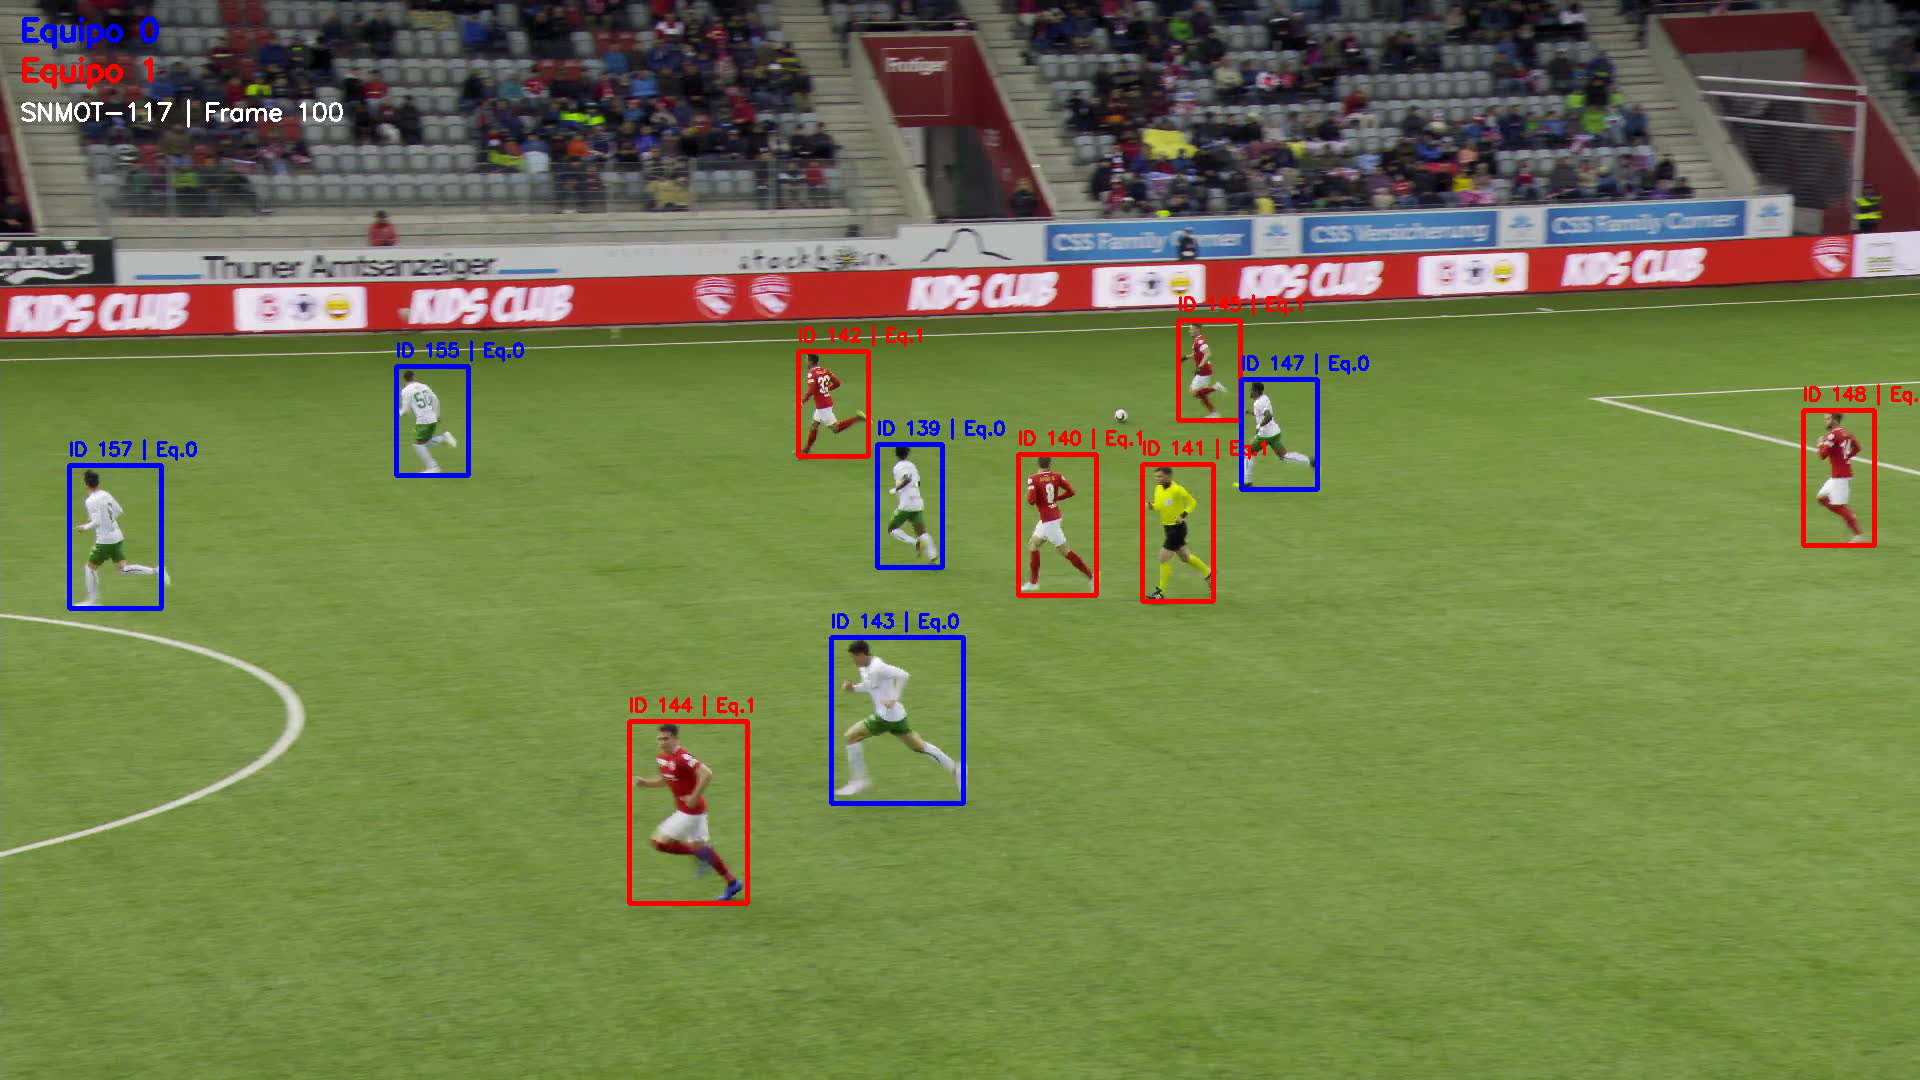
\includegraphics[width=0.85\textwidth]{figures/pruebas_teams_ejemplo.png}
\caption{Clasificación de equipos sobre un frame de
SNMOT-117 (\texttt{team\_visualization.py}).}
\label{fig:pruebas-teams}
\end{figure}

\FloatBarrier

\subsection{Mapas de calor}

La Figura~\ref{fig:pruebas-heatmap} muestra el mapa de calor general
sin homografía, con la proyección aproximada por rango observado
de SNMOT-116, complementario al
mapa de calor por equipo de SNMOT-117 ya mostrado en la
Figura~\ref{fig:diseno-heatmap-ejemplo} del capítulo~\ref{cap:diseno}.

\begin{figure}[htp]
\centering
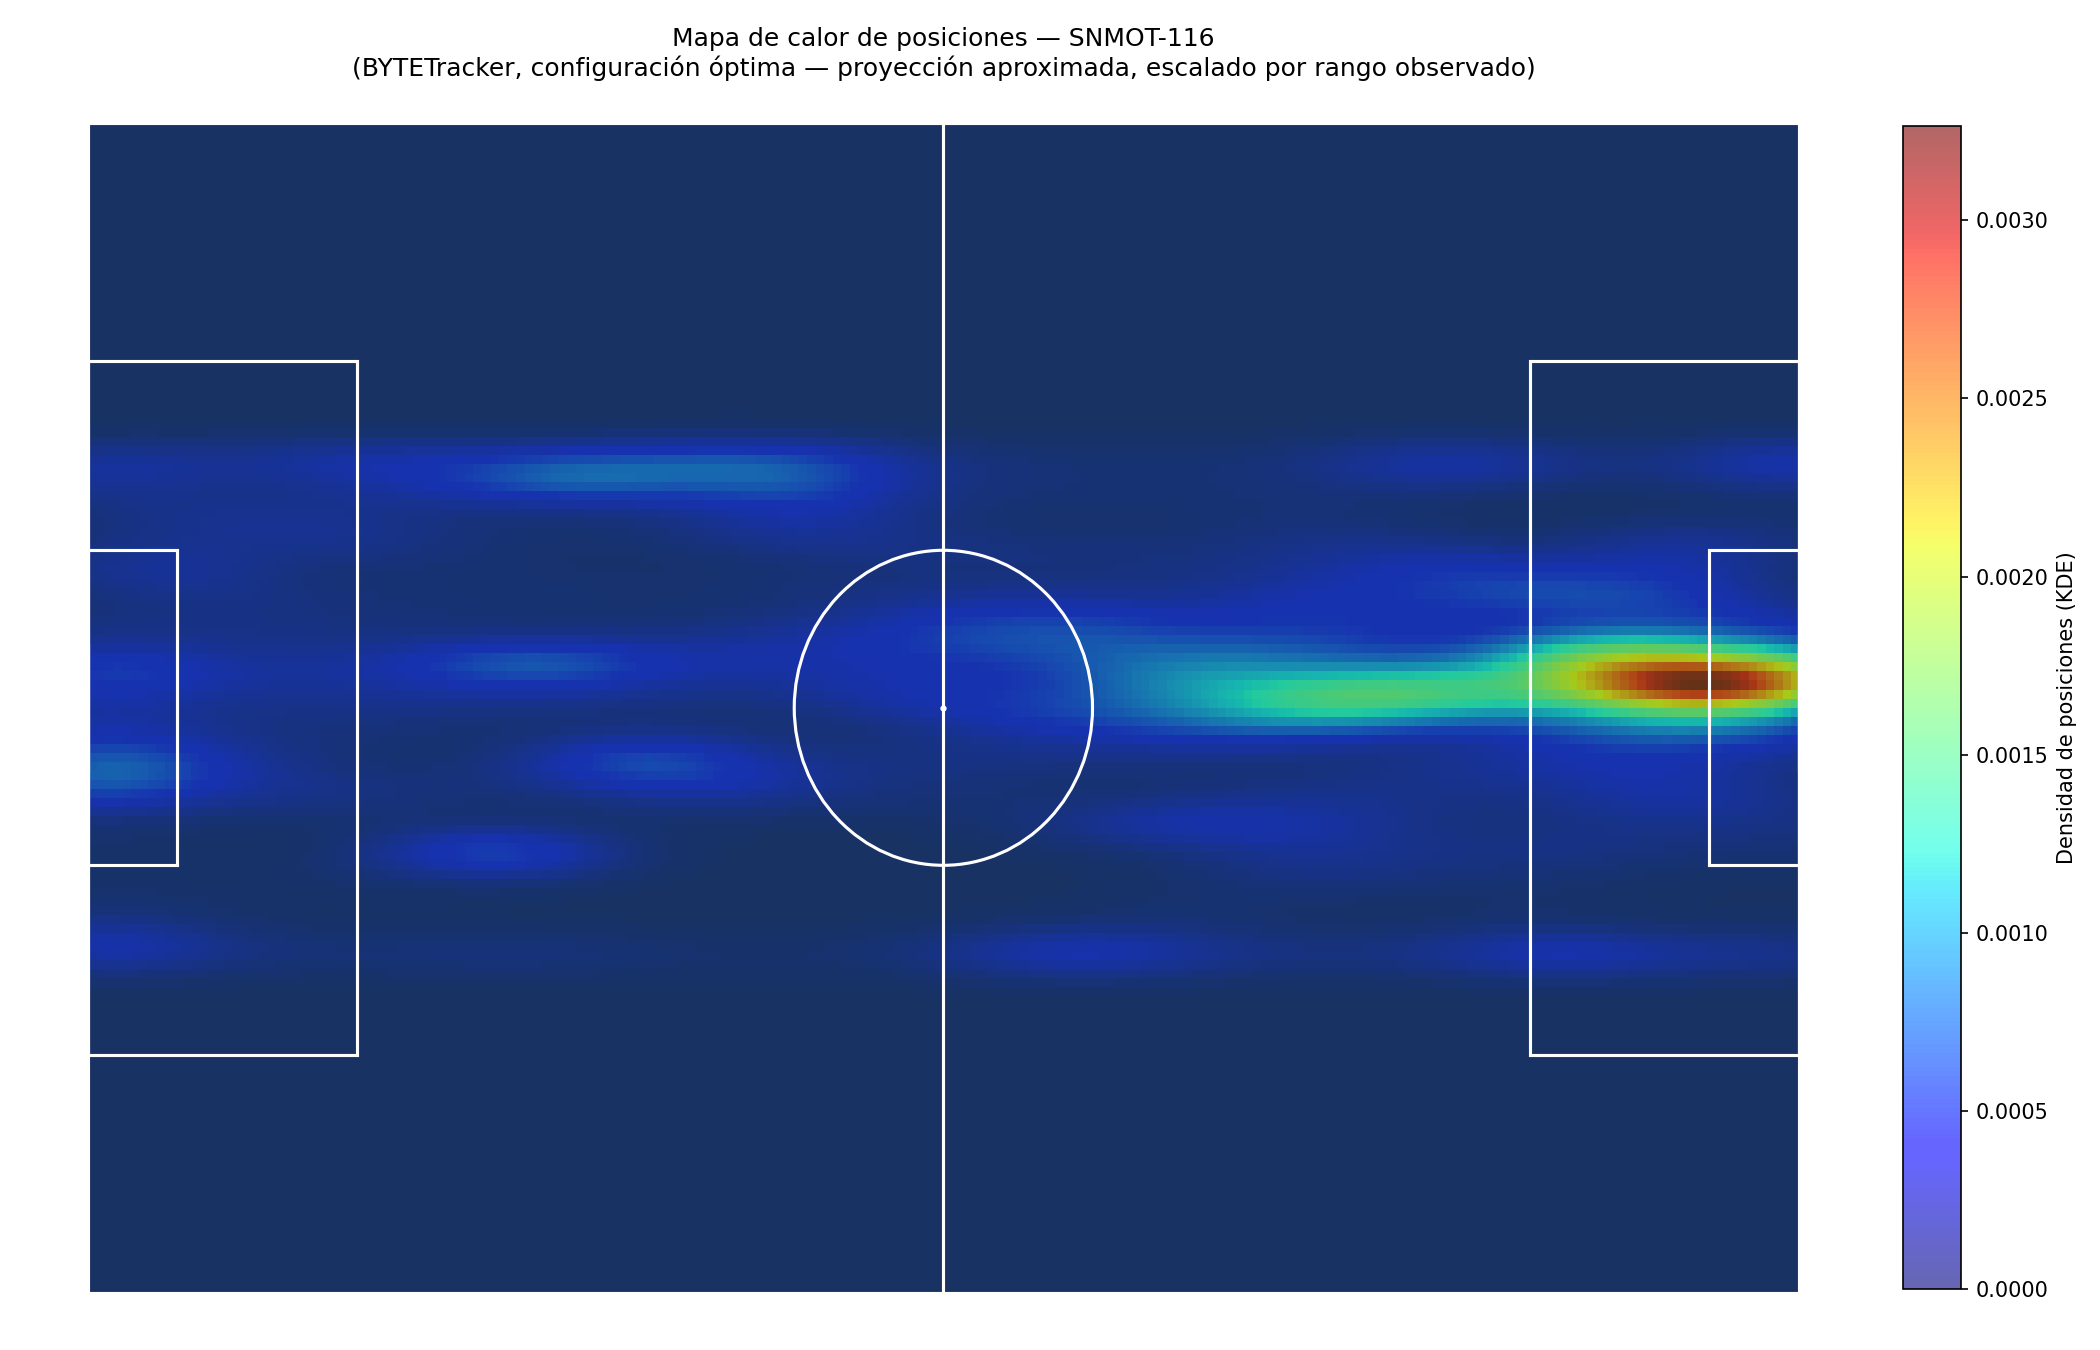
\includegraphics[width=0.85\textwidth]{figures/pruebas_heatmap_field_ejemplo.png}
\caption{Mapa de calor general de SNMOT-116, proyección aproximada sin
homografía.}
\label{fig:pruebas-heatmap}
\end{figure}

\FloatBarrier

\subsection{Distancia y velocidad por homografía}

La Tabla~\ref{tab:pruebas-distancia} recoge los cinco jugadores con mayor
distancia recorrida en cada uno de los dos tramos de demostración
analizados con homografía real.

\begin{table}[htp]
\centering
\caption{Jugadores con mayor distancia recorrida en cada tramo analizado con homografía real.}
\label{tab:pruebas-distancia}
\renewcommand{\arraystretch}{1.25}
\begin{tabular}{|p{2.3cm}|p{1.6cm}|p{2.2cm}|p{2.4cm}|p{2.4cm}|}
\hline
\rowcolor{gray!25}
\textbf{Secuencia} & \textbf{ID} & \textbf{Distancia (m)} & \textbf{Vel.\ media (km/h)} & \textbf{Vel.\ pico p95 (km/h)} \\
\hline
\multirow{5}{*}{SNMOT-116} & 14 & 46{,}81 & 7{,}12 & 21{,}23 \\
\cline{2-5}
 & 13 & 45{,}06 & 7{,}67 & 17{,}42 \\
\cline{2-5}
 & 11 & 41{,}12 & 6{,}46 & 18{,}83 \\
\cline{2-5}
 & 9 & 41{,}07 & 8{,}15 & 17{,}63 \\
\cline{2-5}
 & 8 & 40{,}55 & 7{,}34 & 16{,}73 \\
\hline
\multirow{5}{*}{SNMOT-118} & 279 & 48{,}07 & 12{,}92 & 28{,}76 \\
\cline{2-5}
 & 273 & 33{,}03 & 8{,}68 & 28{,}11 \\
\cline{2-5}
 & 309 & 23{,}18 & 7{,}55 & 13{,}50 \\
\cline{2-5}
 & 335 & 22{,}82 & 6{,}53 & 12{,}16 \\
\cline{2-5}
 & 271 & 22{,}77 & 5{,}67 & 10{,}58 \\
\hline
\end{tabular}
\end{table}

\FloatBarrier

Las magnitudes resultan físicamente plausibles para tramos tan cortos: 25 y
16 jugadores rastreados respectivamente en cada tramo (todos los
\texttt{track\_id} con posiciones dentro de la ventana analizada), con
distancias de hasta 48\,m y velocidades de pico de hasta 28{,}8\,km/h en el
tramo de SNMOT-118, coherentes con un sprint corto durante una jugada
ofensiva. La Figura~\ref{fig:pruebas-heatmap-homografia} muestra el mapa de
calor con homografía real de SNMOT-118, complementario al de SNMOT-116 ya
mostrado en la Figura~\ref{fig:diseno-heatmap-homografia-ejemplo}.

\begin{figure}[htp]
\centering
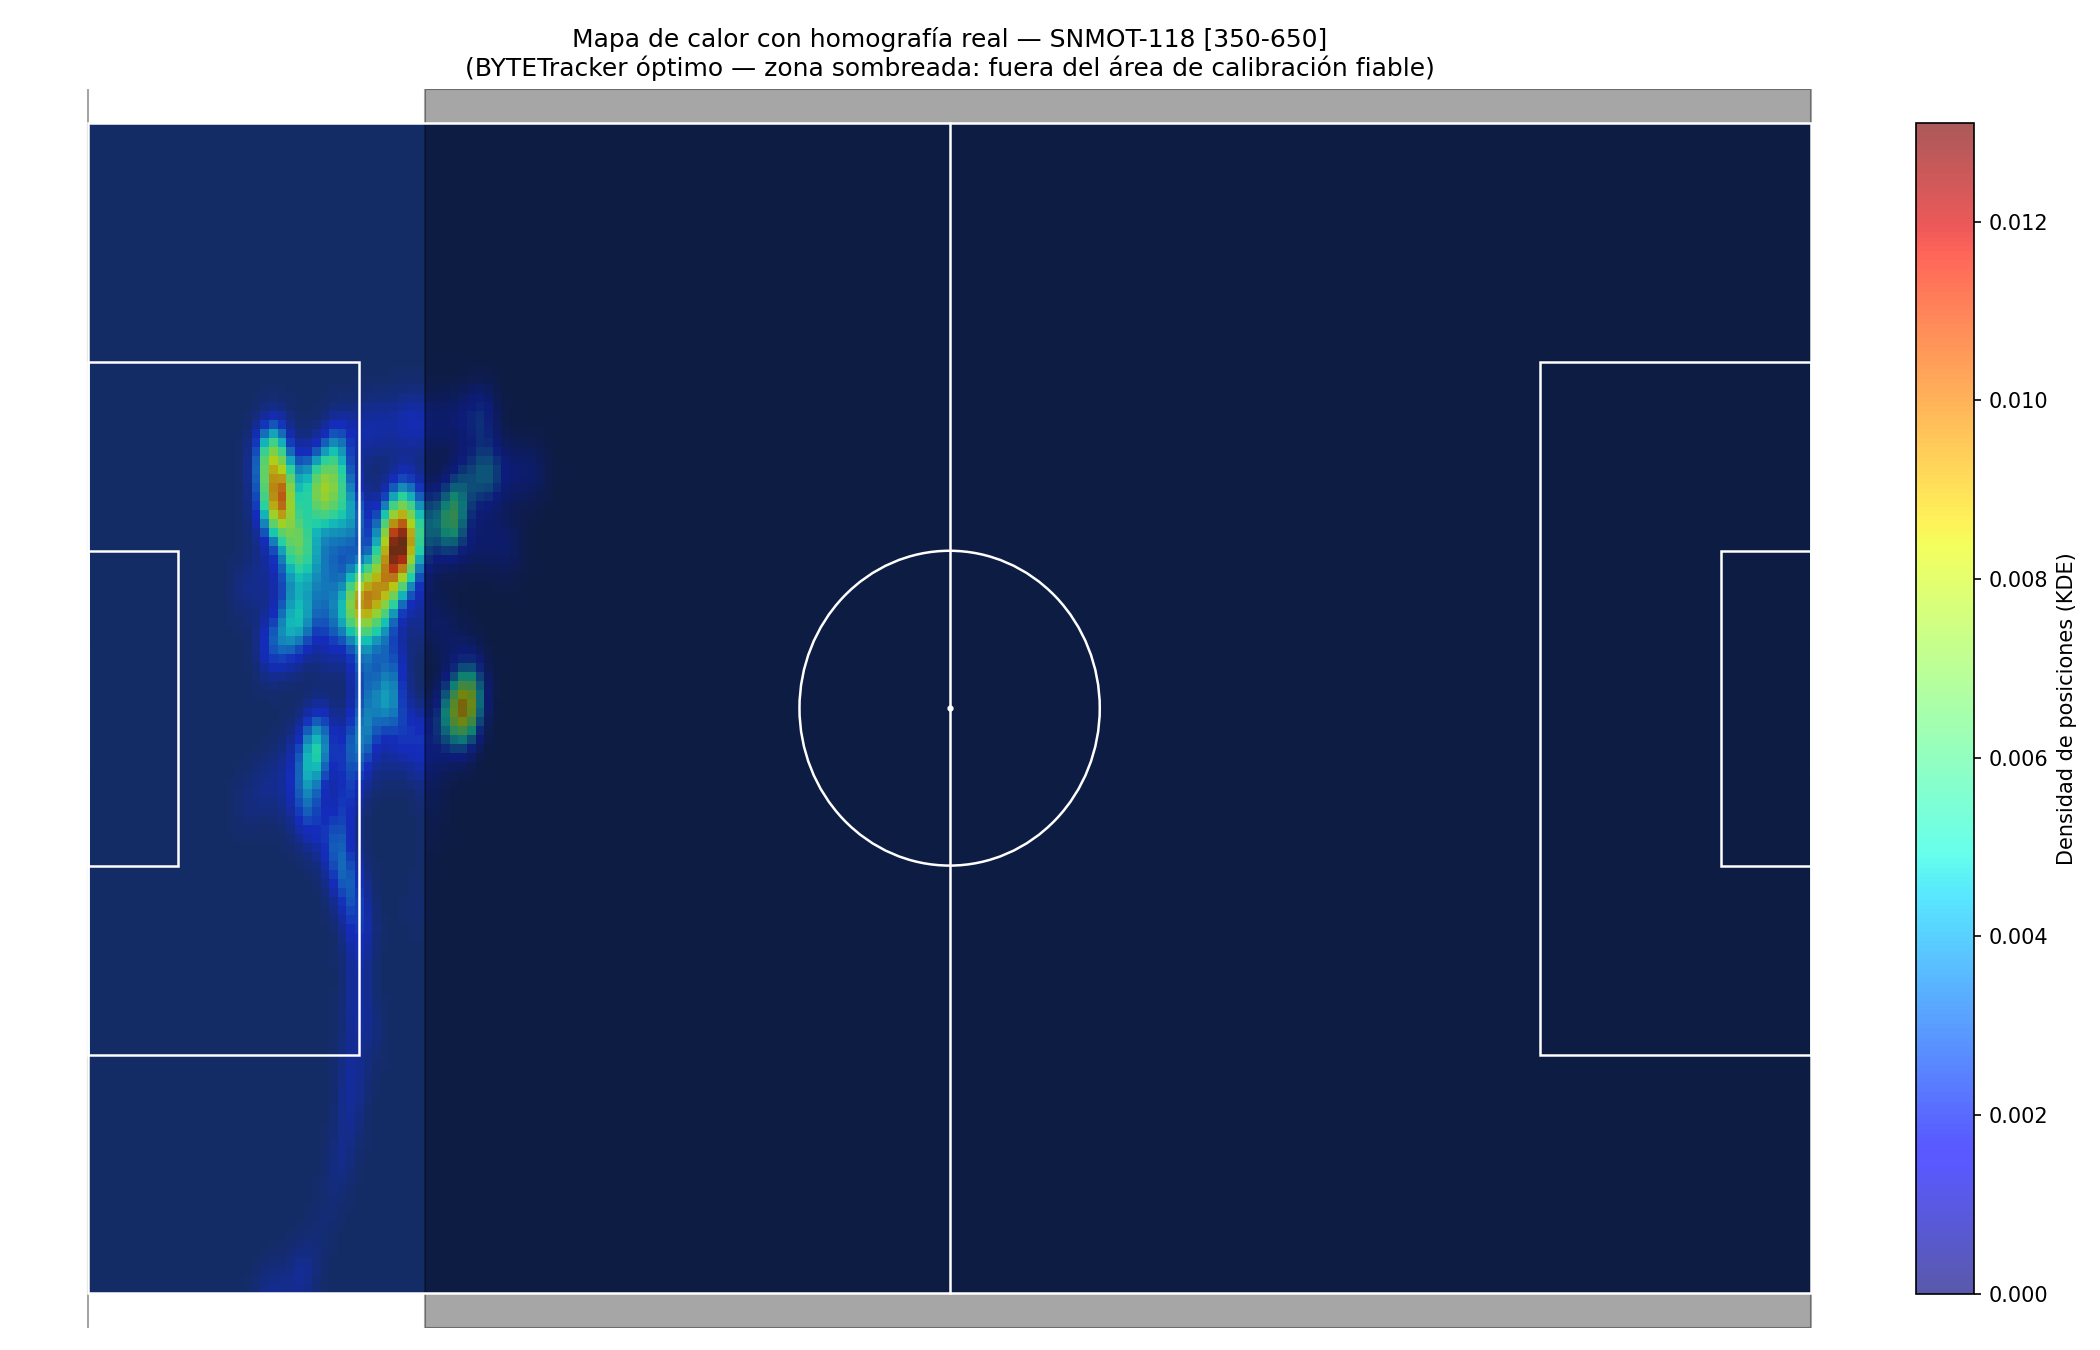
\includegraphics[width=0.85\textwidth]{figures/pruebas_heatmap_homografia_ejemplo.png}
\caption{Mapa de calor con homografía real sobre el tramo de SNMOT-118; la
zona sombreada indica dónde la calibración no es fiable.}
\label{fig:pruebas-heatmap-homografia}
\end{figure}

\FloatBarrier

\subsection{Posesión de balón}

La Tabla~\ref{tab:pruebas-posesion} recoge el porcentaje de posesión por
equipo, estimado por proximidad espacial, en las tres secuencias de
demostración.

\begin{table}[htp]
\centering
\caption{Posesión de balón por equipo y secuencia (estimada por proximidad).}
\label{tab:pruebas-posesion}
\renewcommand{\arraystretch}{1.25}
\begin{tabular}{|p{2.4cm}|p{2.6cm}|p{2.6cm}|p{2.6cm}|}
\hline
\rowcolor{gray!25}
\textbf{Secuencia} & \textbf{Equipo 0} & \textbf{Equipo 1} & \textbf{Frames con posesión asignada} \\
\hline
SNMOT-116 & 85{,}95\,\% & 14{,}05\,\% & 612 \\
\hline
SNMOT-117 & 71{,}81\,\% & 28{,}19\,\% & 667 \\
\hline
SNMOT-118 & 25{,}06\,\% & 74{,}94\,\% & 427 \\
\hline
\end{tabular}
\end{table}

Los repartos obtenidos varían considerablemente de una secuencia a otra
, lo que es consistente con tratarse de tramos
cortos de partido en los que un equipo puede
dominar claramente la posesión del balón durante una jugada concreta sin
que eso sea representativo de la posesión a lo largo de todo el partido.
Como se documentó en el diseño de esta métrica
(sección~\ref{subsec:diseno-posesion}), estos porcentajes deben leerse como
lo que son, una aproximación por proximidad espacial frame a frame y no como una estadística oficial de
partido.

\section{Limitaciones de los resultados}
\label{sec:pruebas-limitaciones}

Al igual que en el resto de esta memoria, conviene cerrar este capítulo
resumiendo las limitaciones que afectan a la validez de
los resultados presentados:

\begin{itemize}
  \item \textbf{HOTA(0) frente a HOTA integrada}: el estudio de
        hiperparámetros completo
        se reporta en términos de HOTA(0), no de la métrica integrada más
        robusta usada en la comparativa principal
        . Recalcular el estudio
        completo con HOTA integrada queda
        como trabajo futuro.
  \item \textbf{Configuraciones óptimas no recombinadas}: no se ha vuelto a
        evaluar la comparativa de HOTA integrada de la
        sección~\ref{sec:pruebas-comparativa} usando las configuraciones
        óptimas de hiperparámetros de cada algoritmo, solo sus valores por
        defecto.
  \item \textbf{Clasificación de equipos sin árbitro}: los porcentajes de
        posesión y los mapas de calor por equipo incluyen al árbitro
        clasificado incorrectamente en uno de los dos equipos, lo que introduce un sesgo
        pequeño en ambos resultados.
  \item \textbf{Homografía real limitada a dos tramos cortos}: los
        resultados de distancia y velocidad se basan en 12-15 segundos de
        vídeo de dos secuencias concretas, no en partidos completos.
  \item \textbf{Posesión como heurística}: los
        porcentajes de la Tabla~\ref{tab:pruebas-posesion} miden proximidad
        espacial al balón, no posesión táctica real, y se calculan sobre
        secuencias muy cortas.
  \item \textbf{Detección del balón por criterio geométrico}: cualquier
        resultado que dependa de la localización del balón tendría
        las limitaciones del filtro geométrico.
\end{itemize}
